\documentclass[b5paper]{report}
\usepackage[left=1cm, right=1cm, top=3cm, bottom=3cm]{geometry}
\usepackage[utf8]{inputenc}
\usepackage{hyperref}
\usepackage{amsmath,amssymb}
\usepackage{pgfplots}
\pgfplotsset{compat=1.9}
% Solves some problems with apalike
\usepackage{natbib}
\usepackage{bm}

%%% New commands JCS
\newcommand{\EE}{\mathbb{E}}
\newcommand{\RR}{\mathbb{R}}
\newcommand{\ptrue}{\boldsymbol{\eta}}
\newcommand{\pest}{{\bf f}} %\newcommand{\pest}{\hat{\boldsymbol{\eta}}}
\newcommand{\loss}{\Psi}   %\newcommand{\loss}{\ell}
\newcommand{\bloss}{\boldsymbol{\loss}}   %\newcommand{\loss}{\ell}
%\newcommand{\argmax}[1]{\underset{#1}{\operatorname{argmax}}~}
%\DeclareMathOperator*{\argmax}{\arg\!\max}

% MPN: Math notation
\DeclareMathOperator*{\Likelihood}{\mathcal{L}}
\DeclareMathOperator*{\Normal}{\mathcal{N}}
\DeclareMathOperator*{\Expectation}{\mathbb{\mathop{E}}}
\DeclareMathOperator*{\Expected}{\mathbb{\mathop{E}}}
\DeclareMathOperator*{\Real}{\mathbb{\mathop{R}}}
\DeclareMathOperator*{\Gradient}{\nabla}
\DeclareMathOperator*{\from}{\sim}
\DeclareMathOperator*{\Kernel}{\mathbf{K}}
\DeclareMathOperator*{\Identity}{\mathbf{I}}
\DeclareMathOperator*{\KL}{\bm{\mathsf{KL}}}
\DeclareMathOperator*{\Jac}{\bm{\mathsf{Jac}}}
\DeclareMathOperator*{\ra}{\rightarrow}
\DeclareMathOperator*{\argmax}{arg\,max}
\DeclareMathOperator*{\argmin}{arg\,min}

% This file contains macros that can be called up from connected TeX files
% It helps to summarise repeated code

%-----------------------------------------------------------------------------
% Figures with caption and description
%-----------------------------------------------------------------------------
\newcommand{\figuremacro}[3]{
% insert a centered figure with caption and description
% Parameters
%   #1: <string> filename
%   #2: <string> caption
%   #3: <string> description
%   #4: <string> label
%
    \begin{figure}[t]
    \centering
    \includegraphics[width=1\linewidth]{#1}
    \caption[#2]{\textbf{#2} #3}
    \label{#1}
    \end{figure}
}

\newcommand{\figuremacroW}[4]{
% insert a centered figure with caption, description and given width
% Parameters
%   #1: <string> filename
%   #2: <string> caption
%   #3: <string> description
%   #4: <float> width
%
	\begin{figure}[htbp]
		\centering
		\includegraphics[width=#4\linewidth]{#1}
		\caption[#2]{\textbf{#2} - #3}
		\label{#1}
	\end{figure}
}

\newcommand{\figuremacroPos}[4]{
% insert a centered figure with caption, description in given position
% Parameters
%   #1: <string> filename
%   #2: <string> caption
%   #3: <string> description
%   #4: <float> pos (e.g. htbp)
%
    \begin{figure}[#4]
    \centering
    \includegraphics[width=.5\linewidth]{#1}
    \caption[#2]{\textbf{#2} #3}
    \label{#1}
    \end{figure}
}


\newcommand{\figuremacroAll}[3]{
% insert a centered figure with caption, description in full page size
% Parameters
%   #1: <string> filename
%   #2: <string> caption
%   #3: <string> description
%
    \begin{figure*}[!t]
    \centering
    \includegraphics[width=1\textwidth]{#1}
    \caption[#2]{\textbf{#2} #3}
    \label{#1}
    \end{figure*}
}

\newcommand{\figuremacroWR}[5]{
% insert a centered figure with caption, description and given width rotated
% Parameters
%   #1: <string> filename
%   #2: <string> caption
%   #3: <string> description
%   #4: <float> width
%   #5: <float> angle
%
	\begin{figure}[htbp]
		\centering
		\includegraphics[width=#4\linewidth, angle=#5]{#1}
		\caption[#2]{\textbf{#2} - #3}
		\label{#1}
	\end{figure}
}

\newcommand{\figuremacroAllWR}[5]{
% insert a centered figure with caption, description in full page with
% particular width and rotated
% Parameters
%   #1: <string> filename
%   #2: <string> caption
%   #3: <string> description
%   #4: <float> width
%   #5: <float> angle
%
	\begin{figure*}[htbp]
		\centering
		\includegraphics[width=#4\textwidth, angle=#5]{#1}
		\caption[#2]{\textbf{#2} - #3}
		\label{#1}
	\end{figure*}
}

%% Example of use of subfiguremacro:
%\begin{figure}
%  \subfiguremacro{figure_1}{}{.5}
%  \subfiguremacro{figure_2}{}{.5}
%  \caption{}
%\end{figure}
\newcommand{\subfiguremacro}[3] {
    \begin{subfigure}[h]{#3\linewidth}
        \centering
        \includegraphics[width=1\linewidth]{#1}
        \caption{#2}
        \label{#1}
    \end{subfigure}
}

%-----------------------------------------------------------------------------
% Figures without caption (common for Beamer slides)
%-----------------------------------------------------------------------------
\newcommand{\figuremacroS}[1]{
% insert a centered figure
% Parameters
%   #1: <string> filename
%
    \begin{figure}[t]
    \centering
    \includegraphics[width=1\linewidth]{#1}
    \end{figure}
}

\newcommand{\figuremacroSW}[2]{
% insert a centered figure of specified width
% Parameters
%   #1: <string> filename
%   #2: <float> width
%
    \begin{figure}[t]
    \centering
    \includegraphics[width=#2\linewidth]{#1}
    \end{figure}
}

\newcommand{\figuremacroSWXY}[4]{
% insert a centered figure of specified width on position x,y
% Parameters
%   #1: <string> filename
%   #2: <float> width
%   #3: <float> x coordinate
%   #4: <float> y coordinate
%
\begin{textblock*}{#2\textwidth}(#3\textwidth,#4\textheight)
	\begin{figure}
		\centering
        \includegraphics[width=1.0\linewidth]{#1}
	\end{figure}
\end{textblock*}
}

\newcommand{\figuremacroSWXYstep}[5]{
% insert a centered figure of specified width on position x,y from given step
% Parameters
%   #1: <string> filename
%   #2: <float> width
%   #3: <float> x coordinate
%   #4: <float> y coordinate
%   #5: <string> steps when to show the figure
%
\begin{textblock*}{#2\textwidth}(#3\textwidth,#4\textheight)
	\begin{figure}
		\centering
        \includegraphics[width=1.0\linewidth]<#5>{#1}
	\end{figure}
\end{textblock*}
}

\newcommand{\posterfigure}[2]{
    \begin{tikzfigure}
    \includegraphics[width=#2\linewidth]{#1}
    \end{tikzfigure}
}

%% YEARS
\newcommand{\marginyear}[1]{\marginpar{\color{red}#1}}
\newcommand{\marginYear}[1]{#1\marginpar{\color{red}#1}}
%% AUTHORS BIBLIOGRAPHY
% \marginauthor{name}{place of born}{years}{description}
\newcommand{\marginauthor}[4]{\footnote{\textbf{#1} (#2; #3) #4}}
\newcommand{\authormark}{\footnotemark{} }
\newcommand{\authortext}[4]{\footnotetext{\textbf{#1} (#2; #3) #4}}
%% It is not possible to put several authormarks in a row
%% it has to be done in the next way:
%% \cite{Rashevsky1938}
% \authormark \authormark \authormark
% \addtocounter{footnote}{-3}
% \stepcounter{footnote}
% \authortext{}{}{}{}
% \stepcounter{footnote}
% \authortext{}{}{}{}
% \stepcounter{footnote}
% \authortext{}{}{}{}

%% FOR epigraphs
\usepackage{epigraph}
\renewcommand{\epigraphsize}{\small\itshape}
\setlength\epigraphwidth{8cm}
\setlength\epigraphrule{0pt}
\newcommand{\myepigraph}[2]{\epigraph{``#1''}{\textup{--- #2}}}


%% For square notes notes
\newcommand{\note}[1]{
\vspace{1ex} \colorbox{black!10}{
  \begin{minipage}{.9\textwidth}#1\end{minipage}}
\vspace{1ex}}

% For corner rounded box
\usepackage{tcolorbox}
\newenvironment{mybox}{
\centering
\begin{tcolorbox}[
    colback=black!10,
    colframe=black!10,
    width=.95\textwidth,
    arc=3mm,
]
}
{\end{tcolorbox}
}


\usepackage{amsthm}
\theoremstyle{plain}
\newtheorem{theorem}{Theorem}[chapter] % reset theorem numbering for each chapter
\theoremstyle{definition}
\newtheorem{definition}[theorem]{Definition} % definition numbers are dependent on theorem numbers



% Adding multiple bibliographies
% See here: https://tex.stackexchange.com/questions/44589/how-to-split-bibliography-for-different-sections
%\usepackage{biblatex}
%\addbibresource{references.bib}
%\printbibliography[title={Rob Fergus}]


\title{Machine Learning Summer School 2018}
\author{Miquel Perello-Nieto}
\date{August 27--September 7, 2018}

\begin{document}

\maketitle
\tableofcontents

\bibliographystyle{apalike}
\bibliography{references}

\chapter{Introduction}

\begin{itemize}
  \item 150 out of 500
  \item Aug 29 19:30 guided tour through downtown Madrid
  \item Sep 1 9:00am Visti to segovia
  \item Sep 5 20:00
\end{itemize}

\chapter{Bayesian Deep Learning: Planting the seeds of probabilistic thinking
by \href{https://shakirm.com/}{Shakir Mohamed}}

- Shakir Mohamed
- Cambridge, CIFAR, DeepMind

\section{Introduction 27 Aug. Mon. 9:30--11:00}

\begin{itemize}
  \item Different views of probability
    \begin{itemize}
      \item Statistical probability: frequency ratio of items
      \item Logical Probability: Degree of confirmation of an hypothesis
          based on logical analysis
      \item Probability as Propensity: probability used for predictions
      \item Subjective probability: probability as a degree of belief
        \begin{itemize}
          \item Probability is a measure of a belief in a proposition given
            evidence. A description of a state of knowledge.
          \item Different observers with different information will have
            different beliefs
        \end{itemize}
    \end{itemize}
  \item $p(x)$ probability of $x$, $p^*(x)$ true probability of $x$
  \item Conditions: $p(x) \ge 0$, $\int p(x) dx = 1$
  \item Bayes rule: $p(z|x) = \frac{p(x|z)p(z>)}{p(x)}$
  \item Parametrisation: $p_\theta(x|z) = p(x|z; \theta)$
  %\item Expectation: $E_{p \theta}(x\z)[f(x;\phi)] = \int p_\theta(x|z)f(x;\phi)dx$
  \item Gradient: missed
\end{itemize}

\begin{itemize}
  \item Generalised Linear Regression
\end{itemize}

\begin{equation}
  \mu = w^T x + b
\end{equation}

\begin{itemize}
  \item Recursive Generalised Linear Regression
  \item Recursively copose the basic linear functions
  \item Gives a deep neural network
\end{itemize}

\begin{itemize}
  \item Probabilistic model
  \item $p(y|x) = p(y|h(x); \theta)$
  \item likelihood function (log of the previous one)
  \item $\mathcal{L}(\theta) = \sum_n \log p(y_n|x_n; \theta)$
  \item Sometimes the likelihood is not computationally tractable because of an
    integral
  \item Likelihoods can give you estimates of parameters
  \item They are efficient estimators, are asymptotically unbiased
  \item It is possible to make statistical tests on the likelihood, this can
    give you confidence intervals
  \item Pool information: combine the outcomes of different data sources
  \item Biggest problem: misspecification, inefficient estiamtes or confidence
    intervals/test can fail completly (assuming Gaussian while data is not)
\end{itemize}

A likelihood function with regularization term

\begin{equation}
  \Likelihood(\theta) = \sum_n \log p(y_n|x_n; \theta) + \frac{1}{\lambda}
\mathcal{R}(\theta)
\end{equation}

Other names for the regularization are \ldots

The Maximum a Posteriory estimation (MAP)

Shows an example of two instantiations for a MAP estimate where the answer
changes from 0 to 1. This problem arises because of the variable scale. In
order to solve that, we need to learn more than just the mean.

In Bayesian analysis there are two core components: the evidence

\begin{equation}
  p(y|x) = \int p(y|h(x); \theta)p(\theta)d\theta
\end{equation}

and the posterior

\begin{equation}
  p(\theta | y,x) \propto p(y|h(x); \theta)p(\theta)
\end{equation}

In Bayesian analysis, all the things that are not obseved need to be integrated
over (averaged out)

\textbf{Intractable Integrals} do not have a closed form, or very
high-dimensional quantities that can't be computed (e.g. using quadrature)

\subsection{Learning and inference}

In statistics there is no distinction between learning and inference, only
inference (or estimation). While in Bayesian statistics, all quantities are
probability distributions, so there is only the problem of inference.

\textbf{TODO Look at this with more detail}

\begin{itemize}
  \item Deep Learning
    \begin{itemize}
      \item Rich non-linear
      \item Scalable learning
      \item Easily composable
      \item negative point
      \item negative point
    \end{itemize}
  \item Bayesian Reasoning
    \begin{itemize}
      \item negative point: Rich non-linear
      \item negative point: Scalable learning
      \item negative point: Easily composable
      \item positive point
      \item positive point
    \end{itemize}
\end{itemize}

Some additional examples of Bayesian reasoning combined with Deep learning are
Density Estimation, Decision Making and Reinforcement Learning.

Deep and Hierarchical models can be decomposed into a sequence of conditional
distributions in the form

\begin{equation}
  p(z) = p(z_1|z_2)p(z_2|z_3) \dots p(Z_{L-1}|z_L)p(z_L)
\end{equation}

A list of different models

\begin{itemize}
  \item Directed vs undirected
  \item observed vs unobserverd variables
  \item parametreic vs non-parametric
\end{itemize}

A list of learning principles (Statistical inference)

\begin{itemize}
  \item Direct
    \begin{itemize}
      \item Laplace approximation
      \item Maximum likelihood
      \item maximum a posteriori
      \item variational inference
      \item cavity methods
      \item integr. nested laplace approximation
      \item expectation maximisation
      \item markov chain monte carlo
      \item noise contrastive
      \item sequential monte carlo
    \end{itemize}
  \item Indirect (missing these ones)
\end{itemize}

Question about calibrated probabilities. In general in classification it is not
but in healthcare is an example of aplication where this is important.

\section{Inferential questions: Mon. 11:30--13:00}

Evidence estimation

\begin{equation}
  p(x) = \int p(x,z)dz
\end{equation}

Moment computation

\begin{equation}
  \Expectation [f(x) | x] = \int f(z)p(z|x) d z
\end{equation}

Identity trick to compute unobserved variables?

Integral problem

\begin{equation}
  p(x) = \int p(x|z)p(z)dz
\end{equation}

Probabilistic one

\begin{equation}
  p(x) = \int p(x|z)p(z)\frac{q(z)}{q(z)}dz
\end{equation}


Importance sampling: Monte carlo estimator

\begin{equation}
  p(x) = \frac{1}{S} \sum_s w^{(s)} p(x|z^{(s)})
\end{equation}

\begin{equation}
  w^{(s)} = \frac{p(z)}{q(z)} \dots
\end{equation}

\subsection{Hutchinson's Trick}

Example with computing the trace of a matrix, KL between two gaussians,
gradient of a log-determinant

The trace problem $Tr(A)$ with zero mean unit variance $\Expected[zz^T] = I$.
Applying the identity trick we obtain

\begin{equation}
Tr(AI) = Tr(A \Expected[zz^T])
\end{equation}

With linear operations allow us to obtain

\begin{equation}
\Expected[Tr(Azz^T)]
\end{equation}

And because of the trace property

\begin{equation}
\Expected[z^T Az].
\end{equation}

Then, with montecarlo methods the expected value is converted into a sumation

\subsection{Probability Flow Tricks}

Given a distribution and sample


\begin{equation}
  \hat{x} \from p(x)
\end{equation}

With a transformation

\begin{equation}
  \hat{y} = g(\hat{x};\theta)
\end{equation}

Change of variables

\begin{equation}
  p(y) = p(x) \left| \frac{dg}{dx}\right|^{-1}
\end{equation}

Example: compute the

\begin{equation}
  \log \det \left( \frac{\partial f(z)}{\partial z}\right)
\end{equation}

This method is seen in the literature as \emph{Normalising Flows} (see more in
the \href{http://akosiorek.github.io/ml/2018/04/03/norm_flows.html}{blogpost})

\subsection{Stochastic Optimization}

Compute the gradient of the common problem

\begin{equation}
  \nabla_\phi \Expected_{q_\phi(z)} [f_\phi (z)] = \nabla_\phi \int q_\phi (z) f_\phi(z) dz
\end{equation}

With some reparametrisation tricks a distribution can be expressed as a
transofmration of other distributions

\begin{equation}
  z \from q_\phi(z)
\end{equation}

Other names for these methods are samples, one-liners and change-of-variables

\subsection{Pathwise Estimator}

Also known as Unconscious statistician, stochastic backpropagation,
perturbation analysis, reparametrisation trick, affine-independent inference.

When to use this trick

\begin{itemize}
  \item Function $f$ is differen
  \item Density $q$ is known with a suitable transorm of a simpler base
      distribution: inverse CDF, location-scale transform, or other co-ordinate
      transform
  \item Easy to sample from base distribution
\end{itemize}

\subsection{Log-derivative trick}

Score function is the derivative of a log-likelihood function

\begin{equation}
  \Gradient_\phi \log q_\phi(z) =
\end{equation}

\subsection{Score-function estimator}

Also known as Likelihood ratio method, reinforce and policy gradients,
automated and black-box inference

We should use this method when

\begin{itemize}
  \item Function is not differentiable, not analytical
  \item Distribution $q$ is easy to sample from
  \item Density $q$ is known and differentiable
\end{itemize}

\subsection{Evidence Bounds}

Integral problem

\begin{equation}
  p(x) = \int p(x|z)p(z) dz
\end{equation}

Proposal

\begin{equation}
  p(x) = \int p(x|z)p(z) \frac{q(z)}{q(z)} dz
\end{equation}

Importance weight

Jensen's inequality

Lower bound: evidence ower bound

\begin{equation}
  \Expected_{q(z)} [\log p(x|z)] - KL[q(z) || p(z)]
\end{equation}

\subsection{Density Ratio Trick}

The ratio of two densities can be computed using a classifier of using samples
drawn from the two distributions. (TODO there is a type here, find out why)

\begin{equation}
  \frac{p^*(x)}{q(x)} = \frac{p(y=1|x)}{p(y=-1|x)}
\end{equation}

\section{Unsupervised Learning Thu. 9:30--11:00}

\begin{itemize}
  \item Move beyond of associating inputs to outputs
  \item Generative models
  \item It allows to perform density estimation
    \begin{itemize}
      \item Probabilistic models
      \item High-dimensional data
      \item Data distribution is targeted
    \end{itemize}
\end{itemize}


Some examples of aplications for generative models is the compression of images
with high resolution GANs. Some artists used GANs to create pieces of video
art. In an example the artist makes a video of a piece of cloth and gives the
video as an input to a GAN that is trained with a particular set of images (eg.
waves on the sea, or fire), then the GAN needs to generate new images that
resemble the training data.

Types of generative models are:

\begin{itemize}
  \item Fully-observed models
  \item Latent variable models (where there is a direction (from z to x?)
  \item Undirected models: where there is no known direction from the
    observed variables X to the hidden variables Z
  \item \href{Sum-product networks}{https://arxiv.org/abs/1202.3732}
\end{itemize}

Some points to consider when designing a generative model

\begin{itemize}
  \item Data: binary, real-valued, nominal, strings, images
  \item Dependency: independent, sequential, temporal, spatial
  \item Representation: continuous or discrete
  \item Dimension: parametric or non-parametric
  \item Computational complexity
  \item Modelling capacity
  \item Bias, uncertainty, calibration
  \item Interpretability
\end{itemize}

\subsection{Fully-observed models}

This are models that operate on the observed data directly. It does not assume
any hidden variables that may interact with our observed variables. As an
example, Markov models assume a dependency with past events, depending on the
number of dependencies with past events it has different orders of dependency.

\begin{align}
  x_1 \from \text{Cat}(x_1|\pi) \\
  x_2 \from \text{Cat}(x_2|\pi(x_1)) \\
  \dots \\
  x_i \from \text{Cat}(x_i|\pi(x_{< n})) \\
  p(x) = \prod_i p(x_i|f(x_{< i}; \theta))
\end{align}

Some of the properties of these models are

\begin{itemize}
  \item Can directly encode how observed points are related
  \item Any type of data can be used
  \item \dots
\end{itemize}

Directed and discrete: NADE, EoNADE\dots
Directed and continuous: Normal means\dots
Undirected and discrete:\dots
Undirected and continuous:\dots

\subsection{Latent variable models}

These models introduce unobserved local random variables that represent a
hidden cause. One of the most common assumptions is to assume some random
hidden noise in the called Prescribed models. On the other hand, \dots.

An example of a prescribed model is a Deep Latent Gaussian Models in wich all
the hidden variables follow a Gaussian distribution that are connected one to
each other and with dependencies to
previous variables.

\begin{align}
  z_3 \from \Normal(0, \Identity) \\
  z_2 \from \Normal(\text{some dependency on}z_3) \\
  z_1 \from \Normal(\text{some dependency on}z_3 \text{and} z_2) \\
  \dots \\
  x_1 \from \Normal(\text{some dependency on}z_{i})
\end{align}

Some of the properties of Latent variable models are

\begin{itemize}
  \item \dots
\end{itemize}

Some dimensions in order to separate different latent models are, discrete vs
continuous, deep vs direct/linear, and parametric vs non-parametric. Some
examples are Buffet process, Sigmoid Belief Nets, Deep Gaussian processes,
Hidden Markov Model, Sparse LVMs, Nonlinear factor Analysis.

\subsection{Implicit Models}

These are models that asume a random hidden variable that adds noise to the
observed variables. One of the most common examples is to assume random
Gaussian noise in a signal.

TODO the following equations need to be checked:

\begin{align}
  z \from \Normal(\mu, \sigma^2) \\
  x \from f(z)
\end{align}

Some of the important properties are

\begin{itemize}
  \item Easy to sample
  \item easy to compute expectations
  \item Can exploit on large-scale classifiers and Convolutional networks
        (I think this is the regularisation part?)
\end{itemize}

We can separate this models mostly on functions discrete time and difffusions
in continous time.

\section{Model-Inference-Algorithm}

We will understand VAriational Autoencoders and Generative \dots

\section{Variational Inference}

The variational principle is a general family of methods for the approximation
of a complicated density by a simpler class of densities. In most of the cases
we can asses the similarity between our approximated distribution and the
original one by using the Kullback–Leibler divergence.

IN variational inference there is always a variational bound that (Evindence
Lower Bound, a.k.a. ELBO)

\begin{equation}
  F(x,q) = \Expected_{q(z)}[\log p(x|z)] - KL[q(z)||p(z)]
\end{equation}

\section{Mean-Fields}

These methods assume that the distribution is factorised (the hidden variables
are independent). This means that we can compute their probability by
multiplying every independent hidden variable probability.


The most expresive model with the true posterior would be $q^*(z|x)
\propto p(x|z)p(z)$ (true posterior), in the least expressive side we have $q_{MF}(z|x) =
\prod_z q(z_k)$ (fully-factorised model). There is a huge vairety of models in
between like Hidden Markov models, Autoregresive models, Gaussian processes?

\section{Variational Optimisation}

In the variational Expectation Maximisation consists on an alternating
optimization for the variational parameters and the model parameters (VEM).

\begin{align}
  \phi \propto \Gradient_\phi  \text{missing equation}
\end{align}

In the E-step instead of computing q with every sample of our dataset, we will
simulate the answer with an Inference network $q(z/x)$ that will give us a
sample $z \from q(z/x)$. This may be an encoder or inverser. TODO need to see
this previous paragraph with more detail.

\section{Reinforcement learning as generative models}

\begin{itemize}
  \item An unknown likelihood
  \item not known analytical
  \item something more
\end{itemize}


Applying all the techniques seen in the three lectures it is possible to learn
a policy learning that can be used in reinforcement learning.
\chapter{An Introduction to Gaussian Processes by
\href{http://learning.eng.cam.ac.uk/Public/Turner/WebHome}{Richard Turner}}

Example with a non-linear regression

Start with an example of a multivariate Gaussian

\begin{equation}
  p(y|\Sigma) \propto  \exp (\frac{-1}{2} y^T \Sigma^{-1}y)
\end{equation}

If we condition the probabilities of one variable we obtain Gaussian shaped
distributions as well


\begin{equation}
  p(y_2 | y_1, \Sigma) \propto (\exp (\frac{-1}{2} y^T (y_2 - \mu_0)\Sigma^{-1}y(y_2 - \mu_0))
\end{equation}

TODO: revise previous equation

If we map any sample from the original distribution, it is possible to draw a
line with the x-axis the different variables (variable index), and the y-axis the coordinates.
If the variables are correlated, the lines should be quite horizontal.

In the examples it goes from 2 variables to 20, and show how the farther is the
variable less correlated is to the first variable.

In the example, there is a coviariance matrix with a Gaussian with fixed
variance in the diagonal with the mean going from the first variable to the
last one.

Then, if some of this variables are actual samples (fix values), then the
sampling process should force the other variables to converge to these samples.
(TODO: check if the following equation is an ``l'' or an ``I'')

\begin{align}
  \Sigma(x_1, x_2) = \Kernel(x_1, x_2) + l\sigma_y^2 \\
  \Kernel(x_1, x_2) = \sigma^2e^{-\frac{1}{2l^2}(x_1 - x_2)^2}
\end{align}

I a non-parametric method  (infinit parameters)

\begin{align}
  p(y|\theta) = \Normal(y;0,\Sigma) \\
\end{align}

where $\sigma^2$ is the scale (vertical scale), and $l$ is the horizontal-scale
(this scales can be seen in the previous lineplot).

In a parametric model

\begin{align}
  y(x) = f(x;\theta) + \sigma_y \epsilon \\
  \epsilon \from \Normal(0,1)
\end{align}

Definition of a Gaussian process: generalisation of a multivariate Gaussian
distribution to infinitely many variables

A Gaussian distribution is fully specified by a mean vector, $\mu$ and a
covariance matrix $\Sigma$.

\begin{equation}
  f = (f_1, \dots, f_n) \from \Normal(\mu, \Sigma) \text{, indices } i=1,
  \dots, n
\end{equation}

\begin{align}
  y(x) = f(x) + \epsilon \sigma_y \\
  p(\epsilon) = \Normal(\epsilon; 0, 1)
\end{align}

place a GP prior over the non-linear function

\begin{align}
  p(f(x)|\theta) = GP(f(x); 0, K_\theta(x,x')) \\
  \Kernel(x, x') = \sigma^2 \exp \left( - \frac{1}{2l^2} (x - x')^2\right)
\end{align}

sum of a Gaussian variable into a GP is still a multivariate gaussian.

\begin{equation}
  \text{missing equation}
\end{equation}

The marginalisation property of Gaussian distributions is

\begin{align}
  p(y_1) = \int p(y_1, y_2) dy_2 \\
  p(y_1, y_2) = \Normal \left( \left[ \right] \text{missing} \right) \rightarrow p(y_1) =
  \Normal(y_1: a, A)
\end{align}

How do twe make a prediction

\begin{align}
  p(y_1 | y_2) = \frac{p(y_1, y_2)}{p(y_2)} \\
  \rightarrow p(y_1|y_2) = \Normal(y_1: a + BC^{-1} (y_2 - b), A - BC^{-1}B^T)
\end{align}

Where $y_1$ are the predicted positions and $y_1$ are the samples

The predictive mean (first part of $\Normal$ is linear in the data $=Wy_2$

The predictive covariance (second part of the $\Normal$) ca be interpreted as
the predictive uncertanity = prior uncertainty $A$ - the reduction in
uncertainty $BC^{-1}B^T$.

What are the implications of the hyper-parameters?

\begin{itemize}
  \item $\sigma$ missing implications
  \item $l$ missing implications
\end{itemize}

We can use the probability distributions to represent the plausibility of the
hyper-parameters (uncertainty) given the data

\begin{equation}
  \text{Bayes theorem with posterior probability of data given the parameters}
\end{equation}

Shows an example of modifying the lengh-scale variable $l$ and showing how the
likelihood of the parameter value starts increasing and decreasing, showing a
peak at lenghtscale 2.

\newcommand\gauss[2]{1/(#2*sqrt(2*pi))*exp(-((x-#1)^2)/(2*#2^2))} % Gauss function, parameters mu and sigma

\begin{figure}[h]
  \centering
  \begin{tikzpicture}
  \begin{axis}[every axis plot post/.append style={
      mark=none,domain=-2:10,samples=50,smooth},
  ylabel=likelihood,
  xlabel=lenght-scale,
  width=\linewidth,
  height=5cm,
  axis x line*=bottom, % no box around the plot, only x and y axis
  axis y line*=left, % the * suppresses the arrow tips
  enlargelimits=upper] % extend the axes a bit to the right and top
  \addplot {\gauss{2}{1.2}};
  \end{axis}
  \end{tikzpicture}
  \caption{Likelihood of the data guiven the value of the lenght-scale $l$}
\end{figure}

\section{Covariance functions}

Warning. Difficult to compare different models. If you try to compute the posterior
probability of the different models guiven the data, it is hard to compute, it
needs approximations and the results are really sensitive to the priors.


\subsection{References}

\begin{itemize}
  \item Gaussian Processes for Machine Learning, Rasmussen and Williams, 2006
  \item \href{http://gpss.cc/}{Gaussian Process Summer School}, Neil Lawrence and collegues
    \item Software
      \begin{itemize}
        \item GPy: Gaussian processes in Python
        \item GPflow: Gaussian Processes and tensorflow
        \item GPML: Gaussian Processes in Matlab
        \item GP Stan: Gaussian Processes in probabilistic programming
      \end{itemize}
\end{itemize}

\section{Using Gaussian Processes: Models, applications and connections
16:30--18:00}

Question 1: Addition of two GPs

\begin{align}
  f(x) = f_1(x) + f_2(x) \\
  f_1(x) \from GP(0, \Sigma_1(x,x')) \\
  f_2(x) \from GP(0, \Sigma_2(x,x'))
\end{align}

The expected value is

\begin{align}
  m(x) = \Expected(f(x)) =& \Expected(f_1(x) + f_2(x)) \\
  =& \Expected(f_1(x)) + \Expected(f_2(x))
\end{align}

And the covariance is

\begin{align}
\Sigma(x) =& \Expected(f(x)f(x')) - \Expected(f(x))\Expected(f(x)) \\
=& \Expected\left[\left(f_1(x) + f_2(x'))(f_1(x) + f_2(x')\right)\right] \\
=& \Expected[f_1(x) + f_1(x')] + \Expected[(f_2(x) + f_2(x')] + \Expected[f_1(x) + f_2(x')] + \Expected[(f_2(x) + f_1(x')] \\
=& \Expected[f_1(x) + f_1(x')] + \Expected[(f_2(x) + f_2(x')]
\end{align}

More generally: GPs closed under linear transofmration / combination:

\begin{itemize}
  \item GP multiplied by a deterministic function = GP
  \item derivatives of GP = GP
  \item integral of a GP = GP
  \item convolution of a GP by a deterministic funtion = GP
\end{itemize}

Question 2: Random linear model

\begin{align}
  g(x) = mx + c \\
  m \from \Normal(0, \sigma_m^2) \\
  c \from \Normal(0, \sigma_c^2)
\end{align}

The expected value

\begin{equation}
  m(x) = \Expected[g(x)] = \Expected(m)x + \Expected(c) = 0 + 0
\end{equation}

The covariance

\begin{align}
  \Sigma(x, x') =& \sigma_m^2 xx' + \sigma_c^2 \\
  =& \Expected(g(x)g(x')) \\
=& \Expected(( mx + c)(mx' + c)) \\
=& \Expected(m^2)xx' + \Expected(c^2) + \Expected(cm)x' + \Expected(mc)x \\
=& \Expected(m^2)xx' + \Expected(c^2) + 0 + 0
\end{align}

Question 3: random sinusoid model

\begin{align}
  h(x) = a \cos(wt) + b \sin(wt) \\
  a \from Normal(0, \sigma^2) \\
  b \from Normal(0, \sigma^2)
\end{align}

\begin{equation}
  m(x) = 0
\end{equation}

\begin{equation}
  \Sigma(x,x') = \sigma^2\cos(w(x-x'))
\end{equation}

Bochner's theorem: Any stationary covariance function can be written as

\begin{equation}
  \Sigma(x - x') = \int \sigma^2 (x) \cos(w(x-x'))dw
\end{equation}

roughly, the function comprises and uncontably infinite sum of random sins and
cosines


\begin{table}[h]
  \def\arraystretch{2.0}
  \centering
  \begin{tabular}{p{.3\linewidth}|p{.3\linewidth}|p{.3\linewidth}}
    linear mappings $f(x) = Wx$ & neural network & Gaussian Process mappings \\
    \hline
    linear regression & neural network regression & Gaussian Process regression \\
    PCA or Factor analysis & variational auto-encoder (VAE) & Gaussian Process latent variable model \\
    Gaussian auto-regressive (or Markov) model & neural auto-regressive density estimation (NADE) & Gaussian process auto-regressive model (GPAR) \\
    linear Gaussian state space model (LGSSM) & recurrent neural latent variable model & Gaussian process state-space model (GP-SSM)
  \end{tabular}
\end{table}

Strenghts of Gaussian Processes

\begin{itemize}
  \item Interpretable machine learning
  \item data-efficient machine learning
  \item decision making
  \item automated machine learning including probabilistic numerics
\end{itemize}

Weaknesses

\begin{itemize}
  \item Large numbers of datapoints ($N \le 10^5$)
  \item High-dimensional inputs spaces ($D \le 10^2$)
\end{itemize}

In the speakers opinion, GPs are not good for large image recognition tasks,
but for small tasks where it is cruciall to get uncertainty estimates.

Example of an Interpretable \href{https://cloud.google.com/automl/}{auto-ML}: the automatic statistician

Given some airline data it detects four underlying patterns, linearly
increasing factor, a periodicity at every year, some incresing noise.

Shows an example with a video of an inverted pendulum and how in a small number
of iterations (around 7?) a GP is learned.

\subsection{Deep Gaussian Processes}

Allowing non-parametric kernel spaces

\begin{align}
  y(x) = f(x) + \sigma_y \epsilon \\
  \text{missing this part}
\end{align}

with a composition of GPs

\begin{align}
  y(x) = f(g(x)) + \sigma_y \epsilon \\
  f(x) = GP(0, K_f(x,x')) \\
  g(x) = GP(0,K_g(x,x'))
\end{align}

Deep GP may perform automatic kernel design


A Neural Network with one hidden layer and infinite number of units in the
hidden layer is a Gaussian Process Nial 1996

A Neural Network  with multiple hidden layers with infinite number of hidden
units on each layer is also a GP (the variance on the weights need a specific
  variance $\sigma^2/D$ Matthews et al. 2018. The specific variance is the
  reason why with finite number of units the regularisation needs to be
  readjusted and follows the values found by Matheews et al.

\subsection{References}

\begin{itemize}
  \item Gaussian process latent variable models for visualisation of high
    dimensional data by Lawrence
  \item Local distance preservation in the GP-LVM throught Back constraints
  \item the automatic statistician
  \item PILCO: a model-based and data-efficient approach to policy serch
\end{itemize}

\section{Large data and non-linear models Tue. 11:30--13:00}

Shows a few examples of sounds generation using Gaussian Processes.

\section{A brief history of gaussian process approximation}

One of the first approaches was to modify the original samples in a way that
the computational complexity of making exact inference was reduced from $O(n^3$
to $O(n^2)$.

See following publications:

\begin{itemize}
  \item Sparse Gaussian Processes using Pseudo-inputs
  \item Local and global sparse gaussian process approximations
  \item Sparse-posterior Gaussian Processes for general likelihoods
  \item Variational Learning of Inducing variables in sparrse Gaussian
    Processes
  \item Fast Forward selection to speed up sparse Gaussian Process Regression
\end{itemize}

Some examples of Factor graphs

\begin{align}
  p(x_1, x_2, x_3) = g(x_1, x_2, x_3) \\
  p(x_1, x_2, x_3) = g_1(x_1, x_2)g_2(x_2, x_3) \\
\end{align}

Where in the first one all the nodes are connected with one factor (square),
while the second one $x_1$ is only connected to $x_2$ and this one to $x_3$.

Shows an example of a multivariate gaussian where the covariance matrix has
some numbers, and the inverse of the covariance matrix presents some zeros. By
looking at the inverse of the covariance matrix we can see what nodes are
independent guiven the rest (positions whith the value zero).

\begin{align}
  \Normal(x, \mu, \Sigma) \propto& \exp[-1/2 (x- \mu)^T \Sigma^{-1}(x- \mu)] \\
  =& \exp[-1/2 \sum_{i,j}(x_i - \mu_i)\Sigma_{i,j}^{-1}(x_j - \mu_j)] \\
  =& \prod_{i,j} \exp[-1/2 (x_i - \mu_i)\Sigma_{i,j}^{-1}(x_j - \mu_j)] \\
  =& \prod_{i,j} g_{i,j}(x_i, x_j)
\end{align}

The previous equations show that when the inverse of the covariance is 0, the
exponent value goes to one and the multiplicative factors are not affected.


The Kullback-Leibler divergence has the Gibb's inequality property, that means
that $KL(p_1(z) || p_2(z)) \ge 0$ and has the equality at $p_1(z) = p_2(z)$. In
order to prove the previous property apply the Jensen's inequality or
differentiation. It is also Non-symmetric $KL(p_1(z) || p_2(z)) \ne
KL(p_2(z) || p_1(z))$.

\subsection{Fully independent training conditional (FITC) approximation}

\begin{enumerate}
  \item Augment model with $M < T$ pseudo data
    \begin{equation}
      p(f, u) = \Normal(\text{f u, with mean 0 and covariance K})
    \end{equation}
  \item Remove some of the dependencies (results in a simpler model)
  \item Calibrate model (e.g. using KL divergence, many choices)
\end{enumerate}

\begin{itemize}
  \item This method introduces a pareametric bottleneck into a non-parametric
    model
  \item Should we add extra pseudo-data when more data is avilable?
\end{itemize}

\subsection{Variational free-energy method (VFE)}

In this case we want to lower bound the likelihood

\begin{align}
  \Likelihood(\theta) =& \log p(y|\theta) = \log \int df p(y,f|\theta) \\
  =& \log \int df p(y, f|\theta) \frac{q(f)}{q(f)} \ge \int dfq(f) \log
  \frac{p(y,f|\theta)}{q(f)} = F(\theta) \\
  =& \int dfq(f) \log \frac{p(f|y,\theta)p(y|\theta)}{q(f)} = \log p(y|\theta)
  - \KL(q(f)||p(f|y))
\end{align}

\begin{align}
  F(\theta) = \int dfq(f) \log \frac{p(y,f|\theta)}{\text{missing}}
\end{align}

At the end we get a lower bound of the likelihood.

\begin{align}
  F(\theta) =& \int dfq(f) \log \frac{p(y,f|\theta)}{p(f_{\ne u}|u)q(u)} \\
  =& \int dfq(f) \log \frac{p(y|f,\theta)p(f_{\ne u}|u)p(u)}{p(f_{\ne u}|u)q(u)} \\
  =& \int dfq(f) \log \frac{p(y|f,\theta)p(u)}{q(u)}
\end{align}


\begin{figure}[h]
  \centering
  \begin{tikzpicture}
  \begin{axis}[every axis plot post/.append style={
      mark=none,domain=-2:10,samples=50,smooth},
  xlabel=$u$,
  width=\linewidth,
  height=4cm,
  axis x line*=bottom, % no box around the plot, only x and y axis
  axis y line*=left, % the * suppresses the arrow tips
  enlargelimits=upper] % extend the axes a bit to the right and top
  \addplot {\gauss{2}{1.2}};
  \addplot {\gauss{2}{1.2}-0.1};
  \end{axis}
  \end{tikzpicture}
  \caption{Where the {\color{blue}blue line} is the true likelihood and the
    {\color{red}red} line is the approximated $q(u)$}
\end{figure}

They may reduce the time complexity from $O(M^3)$ to $O(NM^2)$, however $N$ is
porportional to $M$ and in certain way is just a small improvement.

Some extra references about approximate inference in GPs:

\begin{itemize}
  \item Sparse online gaussian processes
  \item A unifying view of sparse approximate gaussian process regression
  \item variational learning of inducing variables in sparse gaussian processes
  \item on sparse variational methods and the kullback-leibler divergence
    between stochastic processes
  \item A unifying framework for Gaussian Process Pseudo-Point approximation
    using Power Expectation propagation
  \item Streaming sparse gaussian process aproximations
  \item Efficient deterministic approximate Bayesian Inference for Gaussian
    Process Models
\end{itemize}


and about Deep Gaussian processes:

\begin{itemize}
  \item Deep gaussian processes for regression using approximate expectation
    propagation
  \item Doubly stochastic variational inference for deep gaussian processes
\end{itemize}
%\section{Using GPs: Models applications and connections}

%\section{GPs for large data and non-linear models}

\chapter{Deep Learning by Rob Fergus 14:30--16:00}

``Rob Fergus is an Associate Professor of Computer Science at the Courant
Institute of Mathematical Sciences, New York University. He is also a Research
Scientist at Facebook, working in their AI Research Group. He received a
Masters in Electrical Engineering with Prof. Pietro Perona at Caltech, before
completing a PhD with Prof. Andrew Zisserman at the University of Oxford in
2005. Before coming to NYU, he spent two years as a post-doc in the Computer
Science and Artificial Intelligence Lab (CSAIL) at MIT, working with Prof.
William Freeman. He has received several awards including a CVPR best paper
prize, a Sloan Fellowship \& NSF Career award and the IEEE Longuet-Higgins
prize.'' -- \href{https://cs.nyu.edu/~fergus/pmwiki/pmwiki.php?n=PmWiki.Bio}{Personal
Page from New York University}

\section{Deep Supervised Learning}

\subsection{History of Neural Nets}

The connectionsims started around 40's with Hebb's work, McCulloch and Pitts
and Rosenblatt 50's.

Second era started around 80's with Backpropagation to train multi-layered
networks with the work of Rumelhart, Hinton and Williams. And the architecture
of the Convolutional neural networks by Yann LeCun.

The era of Deep learning starts around 2011 with tasks focused on vision,
speech understanding and natrual language processing. The main ingredients
were (1) supervised training of deep networks with (2) faster GPUs and (3) big
labeled datasets.


\subsection{Deep learning vs traditional approaches}

The traditional approach consists on the hand-designed feature extraction that
may be used by a simple classifier in order to predict the labels of a set of
data. On the oposite hand, deep neural networks are focused on learning useful
feature representations that improve the performance of the model on the
dataset.

From 2010 to 2015 there is a clear decrease on the error rate in the ImageNet
tasks by ussing more complex neural networks. The number of layers goes from 8
layers with the AlexNet in 2012 to 152 layers with the ResNet in 2016.

There are similar jumps in the performance of speech recognition systems. As an
example, in 2015 Baidu0's Deep Speach 2 system used 100 million parameteres in
11 layers of a Recurrent Neural Network. It was trained in around 11.940 hours
of English.

In the task of natural language processing and Machine Translation the work by
Sutskever et al. and Cho et.al 2014. Tests of perplexity show a linear decrease
from 2013?

One of the benefits of Deep learning is that altought there is a huge
computational cost during training, it is really lightweight during deployment.
This means that small devices like smartphones are able to perform real-time
predictions. One example is the detection of cars, road and pedestrians on
self-driving cars.

Other interesting areas where deep learning is being applied are: astronomy,
healthcare (e.g. skin cancer classification, or diabetic retinopathy).

\subsection{Some issues with Deep Learning}

(1) There is a missing theoretical understanding and performance guarantees.
(2) Difficult to inspect the models.
(3) Need lots of labeled data
(4) We are still hand-designing the network architecture (instead of the features).
There are some attempts to learn automatically the architecture (meta-learning)
like Neural architecture search with reinforcement learning.
(5) The most generic architectures (i.e. fully connected) does not seem to
work, and it seems that their architecture is really dependent on the domain
(e.g. for images exploit 2D)

\subsection{Convolutional Neural Networks}

First designed in the work of Yann LeCun (and previously Fukushima) by trying to
mimic the visual system (of cats in Fukushima). It tries to exploit the spatial
relation of pixels. In the work of Fukushima there was no back-propagation and
the architecture could not be learned automatically. It was after
back-propagation was applied into neural networks in 1986 that Yann LeCunn
could show a practical application by classifiying handwritten digits from a
dataset generated by some american post offices with Yann LeCunn as an
investigator (TODO rephrase previous sentence).

If the traditional activation functions were sigmoid shaped like the hyperbolic
tangent or the logistic function, in more recent years activations with linear
regions started to become more popular (e.g. ReLu).

Anothre useful trick is the Batch Normalisation, that has been empirically
proved to improve the performance of CNNs. This method consists on normalizing
the input features with 0 mean and 1 standard deviation on every mini-batch.
There are two extra parameters (TODO missed theses parameters).

\subsection{Stochastic Gradient Descent}

This is an iterative learning method that usually trains with mini-batches.

\begin{equation}
  \text{missing}
\end{equation}

Another training method is the AdaGrad

\begin{equation}
  \theta_{t+1} = \theta_t - \text{missing}
\end{equation}

RMSProp

\begin{equation}
  \text{missing}
\end{equation}

and ADAM

\begin{equation}
  \text{missing}
\end{equation}

\subsection{Some practical debugging tips from M. Ranzato}

\begin{itemize}
  \item Train on small subset of data: the training erro should go to zero
  \item Training diverges: learnoing rate may be too large (decrease learning
    rate), or the back-propagation is buggy because of numerical gradient
    issues.
  \item The parameters collapse, the loss is minimized but the training
    accurayc does not increase: check the loss function
  \item TODO some other tricks missing
\end{itemize}

\subsection{Weights' initialization}

With a simple example with a linear activation with 1 layer neural network we
have

\begin{equation}
  Var[y] = (n^{in}Var[w])Var[x]
\end{equation}

While in a multilayer network

\begin{equation}
  Var[y] = (\prod_d n_d^{in}Var[w_d])Var[x]
\end{equation}

This value during the forward propagation will tend to explode with the depth
$d$. And the backward propagation will make the gradients vanish.

\begin{equation}
  \text{missing derivative of previous equation}
\end{equation}

This makes the initialization really important for a good convergence of the
weights into a good region within reasonable number of epochs (shows empirical
comparison with good and bad initializations).

\subsection{Deep Residual Learning}

It allows some layers to bypass the next layer. This allows the network to skip
layers if these are not necessary for the precition. Empirical experiments show
a decrease from 7.4 error rate (with 34 layers) to 5.7 (with 152 layers).

Some additional information is described in ``Tradeoffs of Large Sclae
Learning, Bottou \& Bousquet, 2011''.


\subsection{Weakly supervised pretraining}

Some recent work on using weakly labeled images from the internet in order to
pretrain deep neural networks.

\href{https://arxiv.org/abs/1511.02251}{Learning Visual Features from Large
Weakly Supervised Data} \cite{Joulin2015}

\section{Unsupervised Learning}

Learning without labels the intrinsic structure of the data. This is
practically important as the real-world categories follow a Zipf's law, meaning
that lots of categories appear very few times.

Some of the benefitrs of unsupervised learning are that there is a vast amount
of free data available, and it is potentially useful as a regularisation
method.

The basic idea is to be able to build a model of $p(X)$ (density modeling)
given just data $\{X\}$.

\subsection{Self supervised learning}

This method consists on using the input data as some part of the target data

\begin{align}
  y: X \rightarrow Y \\
  x \rightarrow y(x)
\end{align}

and use the same techniques used in supervised learning to train a model


\begin{equation}
  \argmin_\theta \frac{1}{n} \sum_{i=1}^n l(f_\theta(x_i), y(x_i))
\end{equation}

This approach usually requires some knowledge of the domain. Some examples are
word2vec in wich the word in the central position of a sentence is considered
the target prediction.

\subsection{Auto-Encoder}

This method tries to find a hidden representation that keeps as much
information of the input data as possible by reducing the reconstruction error.
The network is divided between a decoder and a encoder part.

\subsection{Variational Auto-Encoder}

Similar  to the simple autoencoder but makes


\subsection{Generative Adversarial Networks}

This consists in a decoder-only model but that uses an advesarial loss term
using a discriminator $D$. Mini-max game between G and D.

\subsection{Stacked Auto-Encoders}

The Ladder Networks (Rasmus et al. 2015) adds a reconstruction constrain at
every layer. In this way, there is a loss between every layer that can be
minimized. This is like being able to generate hidden variable states apart
from the input data.

\subsection{Other approaches}

Autoencoders, restricted / Deep Boltzmann Machines, \dots

\subsection{Application examples}

Stochastic video generation (Denton and Fergus 2018) tries to predict the
following frames from a video using encoders, decoders and Long Short Term
Memories. The underlaying method is a Variational Auto-Encoder.

An application example is shown with synthetically generated videos using MNIST
dataset and two bouncing numbers in a closed square. The task of the model is
to predict the position of the numbers in the future (pixel by pixel?). It is
possible to sample from the learned distribution, possibly generating an
un/certainty heat-map.

Training a generative model to add color to images from just their luminance
levels.

Training a generative model to predict the word in the middle of a sentence.

Cut an image into different sections (3x3 squares?) and train a model to
predict to which part of the image every pice belongs to. Unsupervised Learning
of Visual Representations by Solving Jigsaw Puzzles \cite{Noroozi2016}.

Automatic learning of images and audio from videos \cite{Owens2016}. This
method shows how it is possible to know the source of a sound from an image,
some examples show people talking and rainfalls.

Map every image into a hypersphere \citet{bojanowski2017}, hopefully similar
images will fall into nearby regions?

Unsupervised learning of visual representations using videos
\citep{wang2015unsupervised}

\section{Deep Learning Models Rob Fergus 9:30--11:00}

Most of the deep learning models are exploiting some structural bias of the
data. For example, images have a 2D correlation pixelwise, while speech
recognition and natural language processing exploits a 1D time correlation.

\subsection{Memory in Deep networks}

Deep neural networks are not able to store memory to solve sequential problems.
Some networks are able to store implicit internal memory on their connections
like Recurrent Neural Networks and Long Short Term Memory networks.

\subsubsection{Implicit internal memory}

Recurrent neural networks have the computational and the memory integrated in
their weights. However, one of the main problems of RNNs is how to prevent the
network from forgetting during the training. In order to solve that problem
Mikolov et al. 2014 separated the state into a fast and slow changing part.
Other approaches are by using gated units for the internal state like
Long-short term memory (LSTM) (see Hochreiter \& Schmidhuber 1997, Graves,
2013), or Simplified minimal gated unit variations for RNNs. Also GRU
light-weight version from Cho et al 2014.

RNN search: attention in machine translation \cite{bahdanau2014neural}
investigates an encoder and decoder model in a RNN, similar method was used
later for image caption generation with attention \cite{xu2015show}, this last
method allows the network to be queried and create heatmaps on the original
images to correlate the generated words with their corresponding patch.

\subsubsection{External Global Memory}

Some work tries to split the computational memory from the problem solving
memory aspect. These two parts are called the \emph{memory module} and the
\emph{controller module}. The controller is able to write and read to the
memory module. The memory needs some addressing mechanism, and can be soft or
hard. The benefit of soft addressing is that it can be trained by
backpropagation, while the hard addressing is not differentiable.

The end-to-end memory network (MemN2N) \cite{SukhbaatarSWF15} is an
architecture. The memory module is able to store some input vectors and hidden
states, the controller module is able to search in the memory for similar
patterns and obtain the corresponding associated output. This can be a new
hidden state that will be combined with the current hidden state of the
controler.

\begin{enumerate}
  \item Embed each word (word to vector?)
  \item Sum embedding vectors ($v_{Sam} + v_{drops} + v_{apple} = m_i$)
  \item It generates one memory per sentence
  \item The controller takes the vector encoding of the question and makes a
    dots product with the memory sentences and applies a softmax.
  \item This guives weights to each sentence it computes a weighted sum of
      the sentences' representations.
  \item The representation is guiven to the controller and generate an answer
    from it.
\end{enumerate}

Another example is the Neural Turing Machine \cite{graves2014neural} in which
the authors design an end-to-end diferentiable architecture that may be trained
by backpropagation to solve tasks involving memory. Some example applications
are coping, sorting and associative recall of inputs with outputs.

\section{Deep Nets for sets}

There ar problems where there is permuation invariance, dynamic sizong, single
output, or output for each element.

In the Communication Neural Network (CommNet) \cite{sukhbaatar2016} the inputs
and outputs are sets, another example is the DeepSets \cite{zaheer2017deep}.
The CommNet is a special case of a Graph NN in which a set can be represented
as a complete graph.



\chapter{Statistical machine learning and convex optimization by Francis Bach}

\section{Introduction 14:30--18:00}

We will use $n$ for the number of observations and $d$ for de dimension size.
When working with big data we will seek ideally for a running-time complexity
of $O(dn)$.


\section{Classical methods for convex optimization}

In supervised learning we have a set of observations $(x_i, y_i) \in X, Y,
i=1,\dots,n$, i.i.d. (this assumption is almost never true).

For regression $y \in \Real$ and prediction $\hat{y} = \theta^T \Phi(x)$, for
classification $y \in {-1, 1}$ and the prediction is $\hat{y} =
\text{sign}(\theta^T \Phi(x))$.

Empirical risk minimization to find a $\hat{\theta}$ solution to

\begin{equation}
  \argmin_{\theta \in \Real^d} 1/n \sum_{i=1}^n l(y_i, \theta^T \Phi(x_i)) +
    \mu \Omega(\theta)
\end{equation}

the training cost (or empirical risk) is

\begin{equation}
  \hat{f}(\theta) = 1/n \sum_{i=1}^n l(y_i, \theta^T \Phi(x_i))
\end{equation}

and the testing cost or expected risk is

\begin{equation}
  \hat{f}(\theta) = \Expected_{(x,y)}l(y_i, \theta^T \Phi(x_i))
\end{equation}

This imposes two fundamental questions: (1) how are we finding the optimal set
of parameters $\theta$ and (2) how to analyse $\hat{\theta}$.

The loss for a single observation is $f_i(\theta) = l(y_i, \dots$ TODO missing

Jensen inequality says that $g(\Expected(\theta) \le \Expected g(\theta)$

The global definition of convexity if we assume differrntiability is

\begin{equation}
  \forall \theta_1, \theta_2, g(\theta_1) \le g(\theta_2) + g'(\theta_2)^T(\theta_1 - \theta_2)
\end{equation}

With twice differentiable functions $\forall \theta, g''(\theta) \succeq 0$
(positive semi-definite Hessians).

We ideally want a convex problem because the local minimum is the same as the
global minimum, with an optimal condition in $g'(\theta) = 0$. See also the convex
duality and recognizing convex problems in \cite{boyd2004convex}.

\subsection{Lipschitz continuity}

Bounded gradients of g (lipschitz-continuity) if the function g is convex,
differentiable and has a

\subsection{Smoothness and strong convexity}

\begin{theorem}
  A function $g : \Real^d \ra \Real$ is \emph{L-smooth} if and only if it is
  differentiable and its gradient is L-Lipschitz-continuous
  \begin{equation}
    \forall \theta_1, \theta_2 \in \Real^d, ||g'(\theta_1) - g'(\theta_2) ||_2
    \le L||\theta_1 - \theta_2||_2
  \end{equation}
\end{theorem}

Adding a regularization $\mu/2 ||\theta||^2$ with a value of $\mu$ on the order
of $1/n$.

\subsection{Analysis of empirical risk minimization}

most important slide from the first part is summarized in slide 47


\subsection{Accelerated gradient methods (Nesterov, 1983)}

Algorithm

\begin{align}
  \theta_t = \eta_{t-1} - \frac{1}{L}g'(\eta_{t-1}) \\
  \eta_t = \theta_t + \frac{t-1}{t+2}(\theta_t - \theta_{t-1})
\end{align}

with bound

\begin{equation}
  g(\theta_t) - g(\theta_*) \le \frac{2L ||\theta_0 - \theta_*||^2}{(t+1)^2}
\end{equation}

\subsection{Optimization fro sparsity-inducing norms}

See Bach, Jenatton, Mairal, and Obozinski, 2012b \cite{bach2012optimization}.

\subsubsection{Newton method}

Minimize the  second-order Taylor expansion


\subsection{Summary about minimization of convex functions}

\begin{itemize}
  \item Gradient descent: $\theta_t = \theta_{t-1}- \gamma_t g'(\theta_{t-1})$
    \begin{itemize}
      \item $O(1/\sqrt{t})$ convergence rate for non-smooth convex functions
      \item $O(1/t)$ convergence rate for smooth convex functions
      \item $O(e^{-pt})$ convergence rate for strongly smooth convex functions
    \end{itemize}
  \item Newton method: $\theta_t = \theta_{t-1}- g''(\theta_{t-1})^{-1}g'(\theta_{t-1})$
    \begin{itemize}
      \item $O(e^{-p2^t})$ convergence rate
    \end{itemize}
  \item Key insights from Bottou and Bousquet (2008)
    \begin{itemize}
      \item In machine learning, it is not necessary to optimize below
        statistical error
      \item In machine learning the cost functions are averages
      \item Testing errors are more important than training errors
    \end{itemize}
\end{itemize}

\section{Convex stochastic approximation}

There are known global minimax? rates of convergence for non-smooth problems
(Nemirovsky and Yudin, 1983; Agarwal et al., 2012).


\begin{itemize}
  \item Least-squares regression is easy to analyze, and has an explicit
    relationship to bias/variance trade-offs (see Défossez and Bach (2015);
      Dieuleveut et al. (2016).
  \item Many important loss functions are not quadratic (see Bach and Moulines
    (2013)).
\end{itemize}

\begin{figure}[h]
  \centering
  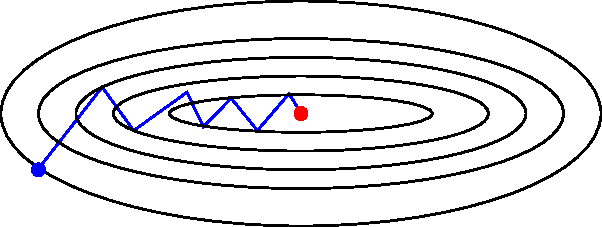
\includegraphics[width=.5\textwidth]{figures/optimization/optimization_batch_gd}
  \caption{Batch Gradient Descent: it needs to decrease the error on every
  step, if not, then the parameters are not right}
\end{figure}

\begin{figure}[h]
  \centering
  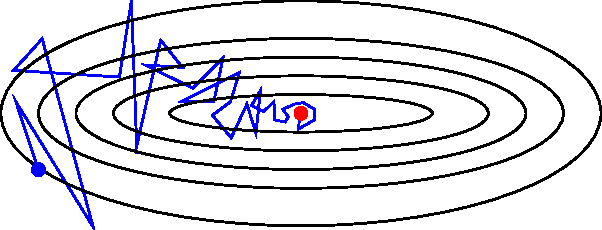
\includegraphics[width=.5\textwidth]{figures/optimization/optimization_stochastic_gd}
  \caption{Stochastic Gradient Descent: the error may increase ocasionally}
\end{figure}

\section{Summary of rates of convergence}

Given the problem parameters

\begin{itemize}
  \item $D$: diameter of the domain
  \item $B$ Lipschitz-constant
  \item $L$ smoothnesss constant
  \item $\mu$ strong convexity constant
\end{itemize}


\begin{table}[h]
  \def\arraystretch{1.4}
  \centering
  \begin{tabular}{|c|c|c|}
    \hline
    & \textbf{convex} & \textbf{strongly convex} \\
    \hline
    nonsmooth & deterministic: $BD/\sqrt{t}$ & deterministic: $B^2/(t\mu)$ \\
              & stochastic: $BD/\sqrt{n}$ & stochastic: $B^2/(n\mu)$ \\
    \hline
    smooth & deterministic: $LD^2/t^2$ & deterministic: $\exp(-t\sqrt{\mu/L})$ \\
           & stochastic: $LD^2/\sqrt{n}$ & stochastic: $L/(n\mu)$ \\
           & finite sum: $n/t$ & finite sum: $\exp(-t/(n+L/\mu))$ \\
    \hline
    quadratic & deterministic: $LD^2/t^2$ & deterministic: $\exp(-t\sqrt{\mu/L})$ \\
              & stochastic: $d/n + LD^2/n$ & stochastic: $d/n + LD^2/n$ \\
    \hline
  \end{tabular}
  \caption{Summary of rates of convergence}
\end{table}

\section{Conclusions}

\begin{itemize}
  \item Statistics with our without optimization
    \begin{itemize}
      \item Significance of mixing algorithms with analysis
      \item Benefits of mixing algorithms with analysis
    \end{itemize}
  \item Open problems
    \begin{itemize}
      \item Non-parametric stochastic approximation (Dieuleveut and Bach, 2014)
      \item Characterization of implicit regularization of online methods
      item Structured prediction
      \item Going beyond a single pass over the data (/testint performance)
      \item Parallel and distributed optimization
      \item Non-convex optimization (Reddi et al., 2016)
    \end{itemize}
\end{itemize}


\chapter{Supervised Learning and Text Classification by Kyunghyun Cho}

\section{Introduction to supervised learning with ANNs Wed.  11:30--13:00}

An overview on supervised learning, in which the input is described as a
validation set $D_{val}$ and a test set $D_{test}$

At the end we need to choose the hypothesis that best adjusts to our problem
between the availables. Examples of hyperparameters sets are in SVMs the
regularization parameters and the kernel, simiarly with Gaussian Processes with
the kernel and the parameters $\sigma^2$ and \emph{lenght-scale}.

In Artificial Neural Networks the hypothesis set is the set of architectures,
and hyperparameters. The architecture is commonly an directed acyclic graph
(DAG) with parameters, inputs, outputs and compute nodes (functions that are
often differentiable).

An example of architecture is a logistic regression where

\begin{equation}
  p_\theta(y=1|x) = \sigma(w^T x + b = \frac{1}{1 + \exp(-w^T x - b)}
\end{equation}

or a 3rd-order polynomial function.

The inference is done by forward propagation of the input to the output trhough
all the hidden layers.

Supervised learning tries to find a function $f_\theta(x)$, while in the case
of Neural Networks we can usually interpret it as computeing the conditional
probabilities guiven the input $p(y='|x)$. This is achieved by computing any
arbitrary output values from a network, then exponentiating every individual
prefdiction and dividing them by their sum (soft-max function).

The objective is that the training data is maximally maximized, by ensuring
that the maximum individual probabilities is maximized at the same time.

\begin{equation}
  \argmax_\theta \log p_\theta(D) = \argmax_\theta \sum_{n=1}^N \log
  p_\theta(y_n|x_n)
\end{equation}

We can also use the log-likelihood

\begin{equation}
  \text{Missing equation}
\end{equation}

\subsection{Loss minimization}

In order to minimize the loss it is necessary to use optimization techniques,
in the case of Artificial Neural Networks (ANNs) is by using backpropagation to
compute the partial derivatives of the parameters with respect the input using
the chain rule of derivatives

\begin{equation}
  \frac{\partial(f o g)}{\partial x} = \frac{\partial f}{\partial
  g}\frac{\partial g}{\partial x}
\end{equation}

This differentiation is done automatically by
\href{https://github.com/HIPS/autograd}{autograd} which will implement the
Jacobian-vector product of each P node.

By doing backpropagation we obtain the gradient of the loss with respect to
every parameter $\theta$. Instead of computing the gradient for the full
dataset, it is common to use mini-batches with a method called Stochastic
Gradient Descent.

\begin{enumerate}
  \item Random subset of M training examples
  \item Compute the minibatch gradient
    \begin{equation}
      \Gradient L \sim 1/N' \sum_{n=1}^{N'} \text{missing part}
    \end{equation}
  \item Update the paraemters $\text{missing equation}$
  \item repeat until the validation loss stops improving
\end{enumerate}

However, this method will find a local minima in the training set, in order not
to overfit to the training data, a validation set is used to do an early stop.
This is one of the most important parts of the training as we want the minima
to be as near as possible to the dataset near.

\section{Text classification}

In text classificatio the input are sentences or paragraphs and the output is a
category to which the input belongs to (commonly a fixed number of $C$
categories).

Some of the particularities of using sentences as imputs is that they are of
variable size $X = (x_1, x_2, \dots , x_T)$ where every $x_t$ is a token from
a vocabulary $V$. This is done by automatically (or manually) splitting all the
individual words and creating an index of words that will form our vocabulary
$V$. Then every sentence is encoded by a sequence of integers. In this case we
are not tokenizing the words first by extracting any meaning of the word, in
this sense the words ``cat'' and ``cats'' have completly independent indices.

At the end the words are encoded as one-hot-encoding with a bit to 1 for the
corresponding index. This will be given to the ANN and will be fordard
propagated to obtain a hidden representation $e_i$. This can be interpreted as
a table lookup from a word to a hidden embedding (eg. a fixed matrix $W$ of
  dimmension $\text{\#tokens} \times \text{\#arbitrary dimesion}$ that is
multiplied by the binary token).

The representation of a sentence is a continuos bag-of-words, this means that
we ignore the order of the words in the sentence, and average the corresponding
token vectors. The method has been proven to be very useful in the works
Iyyer2016, cho2017, and in FastText by Bojanowski2017.

\subsection{How to represent a sentence}

When the order of the words is important, it is possible to encode every set of
words. For example, Relation Network: skip bigrams consider all the possible
pairs of tokens and averages all the relationship vectors. The relations
between words can be encoded depending on the problem, we could consider that
the order of the bigrams is not important, only interested on bigrams of
contiguous words, all the possible pairs, or skip some words.

With the previous idea is possible to use Convolutional Neural Networks in
order to convolve the the ``look up table'' trough the input
\cite{kim2014convolutional}.

The CNN can also represent the bigram representations, and it is possible to
learn a weight vector that will choose how many words are important. Look at
the relation between Relational Networks and Convolutional Neural Networks.

\subsubsection{Self-attention 11:30--13:00}

Self-attention is a generalization of a CNN and RN that is able to capture
long-range dependecies with a single layer. It can also ignore irrelevant
long-term dependencies. Also mention generalization with multi-head and
multi-hop attention.

Using a Recurrent Neural Network we can create an online representation of a
sentence by reading every word and storing their representation in the
recursive hidden representation. This allows a cost of $O(T)$ instead of the
$O(T^2)$ necessary to do all the word pairs.

The representation that is generated by the RNN can encode the representation
of a region of the text given it's context. This can then be feeded to the
previously seen atention model that can learn the weighted sum of the context.

In ``Fully character-level neural machine translation without explicit
segmentation'' \cite{lee2016fully} the authors stack a RNN on top of CNNs.

\section{Natural Language Models}

\subsection{Autoregressive language modelling}

The autoregressive sequence modelling assumes that the past tokens influence
the current token as

\begin{equation}
  p(X) = p(x_1)p(x_2|x_1)\cdots p(x_T|x_1,\dots,x_{T-1})
\end{equation}

this holds true given the conditional distribution assumption.

With this method, an unsupervised method is transormed in $T$ smaller
supervised problems.

One think to keep in mind from a question that was asked is that altough the
marginalisation of $p(X)$ should sum to one, in real cases with RNNs this is
not always true. Possibly because of the parametrization.

The autoregressive sequence modelling can be represented as

\begin{equation}
  p(X) = \prod_{t=1}^T p(x_t|x_{<t})
\end{equation}

In order to score a sentence we can compare the output of the Autoregressive
model for several sentences and use softmax to obtain ``probabilities'' (values
between 0 and 1 that sum to one) for each sentence.

\subsection{N-Gram language models}

Before ANNs were used, the idea about ussing the conditional probabilities was
already used on a smaller scale with N-gram models. In this case the $N$ needs
to be decided in advance.

\begin{align}
  p(x|x_{-N},x_{-N+1},\dots,x_{-1}) = \frac{p(x_{-N},x_{-N+1},\dots,x_{-1}, x)} {\sum_{x \in V}p(x_{-N},x_{-N+1},\dots,x_{-1}, x)}
\end{align}

The process then is to get the dataset and count the frequencies of every
occurrence of the tokens $\dots,x_{N-1}$ followed by all the possible tokens
$x$.

There are two main issues that araise by ussing frequentist N-Grams

\begin{enumerate}
  \item Data sparsity: lack of generalization
    \begin{itemize}
      \item If using a 3-gram model you find 3 words that never happened again,
        the product of probabilities will be zero independently on the rest.
      \item One possible solution is to use smoothing by adding a small
        constant
      \item Another solution is to try with all $n \in \{N,\dots,1\}$
    \end{itemize}
  \item Inability to capture long-term depenfdencies
\begin{itemize}
  \item By choosing a fixed $N$ we may lose long term dependencies.
\end{itemize}
\end{enumerate}

\subsection{Neural N-Gram Language Model}

\cite{bengio2003neural} solved some of the previous issues by using the
hidden representation of a Neural Network instead of the tokens. In the
continuous vector space the similar tokens or phrases are nearby.

Some other work on the same direction is \cite{mikolov2013distributed},
, \cite{pennington2014glove}, \cite{le2014distributed}.

An example of this application is the generalization of sentences that never
happened by realizing that some words share some similarities (eg. numbers). An
example was shown in which sentences with the 2-grams ``three teams'', ``four
teams'' and ``four groups'' are able to generalise to the bigram ``three
groups'' by realizing that three and four share a similar continuous space, and
that before groups there could be a number.

In practice

\begin{enumerate}
  \item Collect TODO missing steps
\end{enumerate}

\subsection{Convolutional Language Models}

Convolutional Neural Networks allow to extend the context size by applying the
convolution through larger parts of the text (see kalchbrenner et al, 2015 and
Dauphin et al 2016, ByteNet by \cite{kalchbrenner2016neural}, PixelCNN,
WaveNet, \dots)

Gated convolutional language model by Dauphin 2016 \cite{dauphin2016language}


\subsection{CBoW Language Models (infinite context)}

The idea is similar to the LM of using averages instead of concatenation.

\subsection{Recurrent Language Models}

An RNN can summarize all the tokens seen until $x$ into a continuous vector
representation Mikolov et al, 2010 \cite{mikolov2010recurrent}.

\subsection{Recurrent Memory Networks}

The work of Tran et al., 2016 \cite{tran2016recurrent} combines RNNs to compress the context into a
continuous vector representation with the attention model that learns the
weighting of the context.

\section{Recurrent Networks and Backpropagation}

Consider the full path from a parameter $\theta$ to the loss $l$. The
backpropagation consists on computing the gradient of the $l$ with respect to
the previous node and multiply by the Jacobian matrix of every step back to the
parameter $\theta$.

\begin{equation}
  \Jac_{h^{t+1}}^{h^t} = W^T \text{diag}(\tanh'(a^t))
\end{equation}

Because the Jaciobians are multiplied by every backpropagation step, this means
that

\begin{itemize}
  \item If $W > 1$ (the upperbound of ) the norm blows up, exploding gradient
  \item If $W < 1$ (the upperbound of) the norm shrinks to zero, vanishing
    gradient
\end{itemize}

\begin{equation}
  || \prod_{t'=t}^{} || \le  || \Jac || \text{TODO missing part}
\end{equation}

\subsection{Gated recurrent units}

These type of networks allow to skip some of the paths in order to avoid the
exploding or vanishing gradient.

\begin{itemize}
  \item Adaptive shortcut:
  \item Candidate update + pruning
  \item Update gate: $u_t = \sigma(W_uh_{t-1} + U \cdots$
  \item reset gate $r_t = \sigma(W_rh_{t-1} + U_rx + b_r)$
\end{itemize}

\subsection{Lessons from GRU/LSTM}

\begin{itemize}
  \item Credit assignment over a long path of computation is difficult
    \item Adaptive shorcut or skip-connection helps avoid credit dilution
      \item Gates are an effective way to focus credit assignment
\end{itemize}

\section{Neural Machine Translation 14:30--16:00}

\subsection{History of machine translation}

The original idea was to get a text from one language, (1) perform a
morphological analysis, (2) a syntactic analysis, (3) semantic analsysis, (4) a
semantic composition and obtein an interlingua text that can be transformed
back to any other language Borr, Hovy and Levin 2006 \textbf{TODO missing
citation}.

Allen 1987 ieee icnn, a brief resurrection of Neural Networks in 1997 by
Castano and Casacuberta 1997 \cite{castano1997machine}, then in 2006 Schwenk
2006 \cite{schwenk2006continuous} as a filter source to SMT to ANN to target sentence, then Devlin 2014 from
source to SMT + ANN to target sentence, then source to ANN to target sentence.

\subsection{Encoding: Token representation}

First it is necessary to build a source and target vocabulary of unique tokens
(for each language). Then transform the text into the set of tokens. Then
encode the token sentences into sentence representation vectors, being careful
not to compress the sentences into small vectors that may lose useful
information.


\subsection{Decoding: conditional language modeling}

Using autoregressive networks we are interested in predicting the posterior
probability

\begin{equation}
  p(Y|X) = \prod_{t=1}^T p(y_t|y_{t-1}, X)
\end{equation}

Look at the RNN Neural Machine Translation by Bahdanau et al., 2015
\cite{bahdanau2014neural}. The model uses the target sentence (and what has
been translated until the current moment) in order to generate the following
prediction.

\begin{enumerate}
  \item Encode: read the entire source sentence to know what to translate
  \item Attention:
  \item Decode:
  \item Repeat 2 to 3 until the end-of-sentence (token) is achieved
\end{enumerate}

This method achieved performance as good as the current state-of-the-art
alternative at the moment phrase-based machine translation (PBMT).

At translation time every predicted word of the sentence had an associated
vector of weights that indicted the source words involved, altough the model
was trained only with pairs of text without any extra supervision. We should
consider that every token of the source sentence is at the same time associated
with a context in its language (see \cite{jean2015montreal}).

\subsection{In practice}

Available frameworks

\begin{itemize}
  \item Nematus \cite{sennrich2017nematus}
  \item OpenNMT-py \cite{opennmt}
  \item FairSeq \cite{gehring2017convs2s}
  \item Sockeye \cite{Sockeye:17}
\end{itemize}

\section{Current and ongoing projects}

Multilingual translation, real-time translation, and character level
translation.

\subsection{Multilingual translation}

A common approach has been to use a pivot language to translate languages
without lots of examples. For example, translate korean to Japanese and then to
English as the corpus between them is larger than the Korean to English.

With this idea, there has been some work to generate a pivot common language
that is automatically learned in an ANN. For example, an encoder/decoder
aproach in \cite{firat2016multi, firat2016zero} creates one encoder per source
and decoder per target, and a model is learned for every pair. Later Johnson et
al, 2016, Ha et al, 2016, Lee et al 2017, and Gu et al, 2018 work on an
Universal \dots

A current limitation is these methods drastically depend on the different
amount of available data in each language. The models start ignoring the less
frequent language. However, if given the same proportions of samples for every
language they may overfit to the less frequent one because of the multiple epochs
run on one language compared to the other.

Some work to solve this problem is being done with Meta-Learning MAML in
\cite{finn2017model}. The difference with multitask learning is that  \dots

Another idea is to create the unsupervised lookup tables to convert word tokens
into continuous vectors ussing big corpus of different languages. In this
manner, words with simmilar meanings will fall into similar regions (see
\cite{artetxe2017unsupervised}). In this case, the overfiting is less probable
to happen as the lookup table is only learning a mapping of tokens to a
continuoius space, but not the translation. Then, the translation model is
trained on top of it.

\subsection{Real-Time Translation (learning to decode)}

learning to translate in real-time with neural machine translation
\cite{gu2016learning}

In order to generate the best translation it is possible to generate several
and then select the most probable one. However, ocasionally it may happen that
after several words are translated the topic changes and the best translation
may be a different one. In order to solve this the Beam Search keeps track of
parallel best translations and is able to switch to another one at any point if
necessary.

\begin{mybox}
\textbf{Exploiting the hidden activation}

In a Deep Neural Network huge information in the hidden layers is usually
discarded in order to predict a class; obtaining at the end a binary
prediction. However, the hidden information has rich information about the
original input that can be exploited.
\end{mybox}

By using the hidden information the performance of several methods was
increased \cite{gu2016learning}.

\chapter{Causality by Joris Mooij}

There are many questions in science that are casual (eg. climatology,
healthcare, \dots).

\section{Introduction}


Causation is not correlation (gives example with chocolate consumption being
correlated with number of nobel prizes in different countries, while there is
no actual correlation between both).

In order to represent causal relations we can use \emph{causal graphs}
(directed graphs) in wich nodes are variables $X_n$ from (a vocabulary?) $V$.
While directed edges indicate that the first variable causes direclty another
variable respect to $V$. An example of a cyclic graph where every adjacent
variable is directly connected to its neighbours is the encoding of standing
domino pieces.

It is possible to modify the \emph{causal graph} with an \emph{intervention},
in the example the domino piece $X_2$ is glued to the floor, removing the
direct connections from other pieces to $X_2$, but possibly keeping a
connection from $X_2$ to the adjacent (in case an external user can still force
$X_2$ to fall).

A \emph{perfect (``surgical'', ``atomic'') intervention} on a set of variables
$X \subseteq V$, is an external enforced change of the system (eg. the
previous example).

A \emph{confounder} is a latent common cause:

\begin{mybox}
  $H$ is a confounder of $X$ and $Y$ if:
  \begin{enumerate}
    \item $H$ causes $X$ directly w.r.t. $\{X, Y, H\}$
    \item $H$ causes $Y$ directly w.r.t. $\{X, Y, H\}$
  \end{enumerate}
\end{mybox}

We will denote latent confounders by \emph{bidirected edges} in a causal graph.

\section{Defining causality in terms of probabilities}

\emph{Simpson's paradox} shows that if we interpret the probabilities as causes
we may make wrong decisions. As an example, shows the recovery rate of a drug
test in which depending on the groups separation the most probable outcome
changes.

\begin{mybox}
\begin{enumerate}
  \item The probability of recovery is higher for patients that took the drug
    \begin{align}
      p(\text{recovery}|\text{drug}) > p(\text{recovery}|\text{no drug})
    \end{align}
  \item For both male and female patients the relation was oposite
    \begin{align}
      p(\text{recovery}|\text{drug, male}) <& p(\text{recovery}|\text{no drug,
      male}) \\
      p(\text{recovery}|\text{drug, female}) <& p(\text{recovery}|\text{no drug,
      female})
    \end{align}
\end{enumerate}
\end{mybox}

\emph{endogenous variables} are binary variables that we are interested in.

\emph{Exogenous variables} are latent, independent binary variables that affect
externally the state of our endogeneous variables.

A \emph{Structureal Causal Model (SCM)}, also knwon as \emph{Structural
Equation Model (SEM)}, is a tuple \dots

There is one Structural equations  per endogenous variable.

\begin{enumerate}
  \item a product of standard measures \dots
  \item a product of standard measures \dots
  \item Measurable mapping \dots
  \item A product probbility measure\dots
\end{enumerate}

An augmented functional graph $G^a(M)$ depicts the exogenous variables while
the functional graph $G(M)$ doesn't.

\begin{mybox}
  If $M$ has no \emph{self-loops}, the causal graph of $M$ is a subgraph of the
  functional graph $G(M)$.
\end{mybox}

\begin{mybox}
\textbf{Definition}

We call the family of sets of probability distributions of the solutions of
$M_{do(l,E_l)}$ \dots
\end{mybox}

some of the previous points are teh basic difference between causal models and
probabilistic models.

We donote a marginalization of the model $M$ with respect two variables $X_2$
and $X_4$ as $M^{\backslash\{2,4\}}$.

See the following extra references \cite{de2013global}, and
\cite{bongers2018random}, \cite{blom2018generalized},
Bongers et al., 2018.


\end{document}

